\section{Descriptive Pattern}
After the definition of Domains, Events, and Patterns, and the ordering relationship between them, it comes possible to understand the definition of Descriptive Pattern(DP).\\
DP is a minimum pattern among those t-support by D.[1]
\begin{definition}
Given a pattern P, if P meets two requirments:\\
P is $\tau$ -supported. 
\begin{displaymath}
|[P]|\geq N_\tau
\end{displaymath}
P is a minimum(most specific) pattern
\begin{displaymath}
\forall P' \in \mathcal{P}|P' \ne P, s.t.P < P'
\end{displaymath}
We call $P$ is a Descriptive Pattern $DP$.
\end{definition}
We have an example to understand the relationship between Patterns and Domains:
\begin{figure}[!h]
\centering
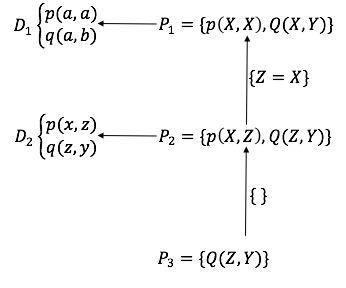
\includegraphics[width=250pt]{./pictures/0303.png}
\caption{Relationship between Patterns and Domains }
\end{figure}
\newpage
From the example, we can see that the variables carry two kinds of information: roles and their fillers:
for example, $P_2$'s $X$ here plays the $l_1 -role$ of $p$, $p(l_1)$.
\begin{table}[!h]
\centering
\begin{tabular}{ccc}
\hline
vars in $P_2$ & role & filler\\
\hline
X & $p(l_1)$ & $a \in D_1$, $x \in D_2$\\
Z & $p(l_2),q(l_1)$ & $a \in D_1$,$z \in D_2$\\
Y & $q(l_2)$ & $b \in D_1$,$y \in D_2$\\
\hline
\end{tabular}
\caption{roles and fillers of variables}
\end{table}
for a pattern P, we can define the role set:[1]
\begin{definition}
Given a variable $X$, and the roles it plays in $\mathcal{D}$,
\begin{displaymath}
role_p (X)={p(l)|p(...,l = X,...) \in P}
\end{displaymath}
is the roles played by $X$.
\end{definition}
$\tau$-supported is the basis condition for patterns to be candidate of $DP$s.\\ \\
\textbf{Least General Generalization}\\ \\
In the initial study of the descriptive pattern, someone have given a method to extract the descriptive pattern from a set of two domains and it can be extended to multi-document situation.
\begin{figure}[!h]
\centering
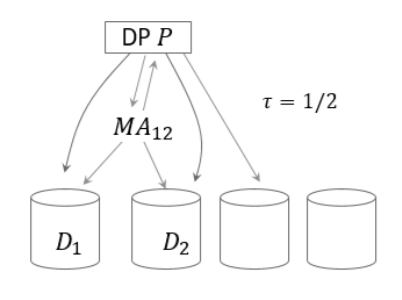
\includegraphics[width=250pt]{./pictures/0303-1.png}
\caption{Least General Generalization}
\end{figure}
That method is called Last General Generalization, LGG.[11] It will generate an indirect value of MA:
\begin{displaymath}
MA_{12} = lgg(D_1,D_2)
\end{displaymath}
From the property of LGG, we will find that $P \preceq MA_{12}$. $MA_{12}$ also meets the the requirment of support $MA_{12}\preceq P$. We can say $P \sim MA_{12}$
From this point,
\begin{displaymath}
DP \iff LGG, LGG\ supported\ by\ N\tau
\end{displaymath}
We can constract DP with LGG with the following method.
\begin{figure}[!h]
\centering
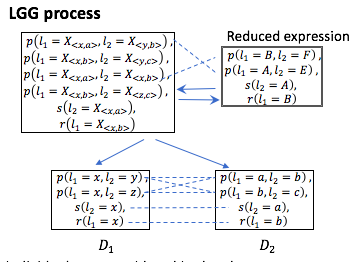
\includegraphics[width=250pt]{./pictures/0303-2.png}
\caption{Least General Generalization}
\end{figure}
For all cases $p(cl)$, we have a sub list of 
$cl_{sub}=\{l_{i_1} = t_{i_1},...,l_{i_n}=t_{i_n}\}$
if we consern 
$p_\{l_{i_1},...,l_{i_n}(t_{i_1},...,t_{i_n})\}$ here, 
$p_l(t)$ 
and $p(l=t)$ have the same meaning. For a event set $Q$, we have $exp(Q)\iff Q$ as all the expend events.
\begin{fact}
$P \preceq D$ by $\theta \iff exp(P)\theta \subseteq exp(D)$
\end{fact}
\begin{definition}
$D_{sel}$: corresponding to $D$ and $\tau$, the set extracted from $N\tau$ domains.
\end{definition}
From that point $lgg(D_{sel})$ is defined as $lgg({exp(D_1),...,exp(D_{N\tau })})$
\\
For a situation of $N\tau > 2$, we will build $N\tau - tuple$ for them as the figure shows,
\begin{figure}[!h]
\centering
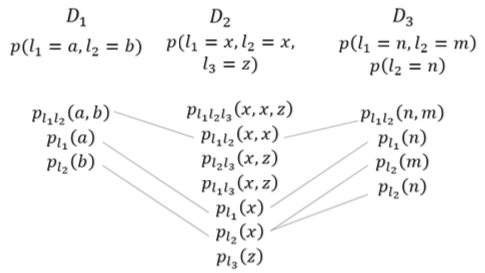
\includegraphics[width=250pt]{./pictures/0303-3.png}
\caption{$N\tau$ = 3 situation}
\end{figure}
For two domains, the pairs of events or individuals are considered in the above construction.
For more than three domains under minimum support parameter less that 1, we need to do consecutive application of LGG or to regard tuples of events/individuals under possible combinations of domains.\\
As the connection of lgg will be increase by square growth.We propose to use neither pairs nor tuples. Similarity classes of individuals over domains: frequent closures (intent of formal concepts)
